\section{Developments in \GAP infrastructure: Tools and processes for
  system and package development, quality assurance and release }\label{sec:gap-infra}

As well as developments in the core system and in packages, we have
dedicated considerable effort to improving our infrastructure and
processes.  In this section we describe developments in the technical
processes which support our developers (especially package
developers), connect them to our user community, and aim to ensure the
robustness and quality of the integrated system, something essential
to its use in demanding large-scale computations. Some of the
technical developments (especially around continuous integration) were
reported in D3.8 (Month 36), and some of the associated advocacy
training and support in deliverables D2.2, D2.11 and D2.15. This
section updates and extends those focussed reports, taking a broad
view of our tools and processes and focussing on the visible benefits
of these changes to developers and package authors. In subsection
\ref{sec:uptake} we assess the impact that this work has had on has
had on the developers and package authors.

\subsection{Regression testing}\label{testing}

\emph{Regression testing} %is a software engineering technique which
checks (preferably in an automated way)
that changes and additions to a system do not break functionality that 
worked previously. If a change breaks a test, that is 
a \emph{regression}. In \GAP, regressions may occur
when a change causes an incorrect result, or a crash, or an unwanted error
message; in addition, there may be \emph{performance regressions}
and \emph{memory regressions} where a test becomes slower, or uses
much more memory after a change.

Regression testing has been used by \GAP in one or another form since 
1980s, and by the beginning of the \ODK project, \GAP had established its testing infrastructure
based on a private \href{https://jenkins.io/}{\sf Jenkins} installation
at USTAN, not accessible outside the local network. That was a major limitation,
because sharing test outcomes with other developers and
allowing them to repeat tests in the same environment was cumbersome
and time-consuming with many manual steps.

%\GAP developers came to an understanding 
%that one of the limiting factors (not only for the testing, but for
%the \GAP development in general) was that while \GAP is an open source 
%software, it does not follow an open development model and does not
%have a public source code repository, and just before the start of
%the project established a public source code repository for \GAP
%on GitHub at \url{https://github.com/gap-system/gap}. 

%In the duration of the OpenDreamKit project we, together with other
%contributors to the \GAP project, consolidated \GAP development 
%around GitHub and its tool ecosystem.
%Hosting GAP repository on GitHub and eventual establishing of a number
%of other repositories under the gap-system and gap-packages 
%organizations (\url{https://github.com/gap-system} and 
%\url{https://github.com/gap-packages}), and encouraging package authors 
%to follow the same practices (see \url{https://gap-packages.github.io/})
%to find some further packages that are having public source code 
%repositories elsewhere) allowed us to bring our regression testing
%up to the next level.
%
%\TODO{maybe mention that we can break out onto GitLab if GitHub
%changes in some unacceptable way} 
%

With the widespread adoption of open development models by the
\GAP system and package developers and
maintainers, taking place during \ODK, we have also been able to move
to an open regression testing infrastructure, which has enabled us
to substantially improve \GAP development and testing workflows and
develop a more robust system with less effort. For example,
today, anyone who is interested in checking the
status of the \GAP test suite can visit the public dashboard at
\url{https://github.com/gap-system/gap-distribution/} of which a
snapshot is shown in figure~\ref{fig:gap-core-tests}.
This dashboard shows the status of the core system GAP tests,
which are run for every change made to the repository, as well as
package integration tests described below.

The ``status'' lights are actually active buttons, which lead to the
full test reports, held on the public continuous integration platform
\href{https://travis-ci.org/}{Travis CI}. The the ``code coverage''
lights are also buttons and lead to the public
\href{https://codecov.io/}{Codecov} service, where, if you drill down far
enough, you can access reports showing exactly which lines of code in the kernel
and library have, or have not been tested.

This level of open continuous testing has led to huge improvements in
the quality of the system, with far fewer bug reports than previously,
and saved enormous effort in integrating releases.

At the heart of the testing of the core \GAP system is achieved by the
comprehensive test suite. The table in
figure~\ref{fig:test-suite-growth} shows its increase over the period.

% find . -name '*.tst' | wc -l
% find . -name '*.tst' | xargs wc -l
\begin{figure}[!ht]
\begin{center}
\begin{tabular}{| l | l | c | c | c |} 
\hline
GAP release & Release date & Number of        & Number of lines & Code coverage \\
            &              & test files       & in test files   &               \\
\hline GAP 4.7.8  & November 2015 (Month 3)   & 69 & 21981 & N/A \\
\hline GAP 4.8.10 & January 2018 (Month 29 )  & 91 & 28586 & N/A \\
\hline GAP 4.9.3  & September 2018 (Month 37) & 564 & 41456 & 69 \% \\
\hline GAP 4.10.2 & June 2019 (Month 46)      & 648 & 53362 & 76 \% \\
\hline GAP 4.11   & November 2019 (planned)   & 707 & 61280 & 84 \% \\
\hline
\end{tabular}
\caption{Growth of the GAP test suite}\label{fig:test-suite-growth}
\end{center}
\end{figure}

In addition, we also test the correctness of the
over $14,000$ lines in the 1810 examples in our manuals.
%% \comment{1336 mansections containing examples;
%% 1641 (ref) + 169 (tut) = 1810 examples;
%% 13262 (ref) + 940 (tut) = 14202 lines}. 
%% in doc/ref
%Read("makedocreldata.g");
%exsref := ExtractExamples(GAPInfo.ManualDataRef.pathtodoc,
%       GAPInfo.ManualDataRef.main, GAPInfo.ManualDataRef.files, "Chapter");;
%exsref := Filtered( exsref, ch -> Length( ch ) > 0 );;
%Sum(List(exsref,Length));
%Sum(List(exsref, ch -> Sum(List( ch, ex -> Length(Filtered(SplitString(ex[1],"\n"), x -> x<>""))))));
%
%% in doc/tut
%Read("makedocreldata.g");
%exsref := ExtractExamples(GAPInfo.ManualDataTut.pathtodoc,
%       GAPInfo.ManualDataTut.main, GAPInfo.ManualDataTut.files, "Chapter");;
%exsref := Filtered( exsref, ch -> Length( ch ) > 0 );;
%Sum(List(exsref,Length));
%Sum(List(exsref, ch -> Sum(List( ch, ex -> Length(Filtered(SplitString(ex[1],"\n"), x -> x<>""))))));
%%
%% 
% and some further code in the {\tt benchmarks} directory. 
%

We promote a similar testing approach to \GAP package authors and
encourage them to provide their own regression
tests. Many do, adding, in total over a quarter of a million lines of
further tests in the distributed system, which are run when new
versions of packages and/or of the core system are being tested for
integration into a release.

\begin{figure}[!ht]
    \centering
    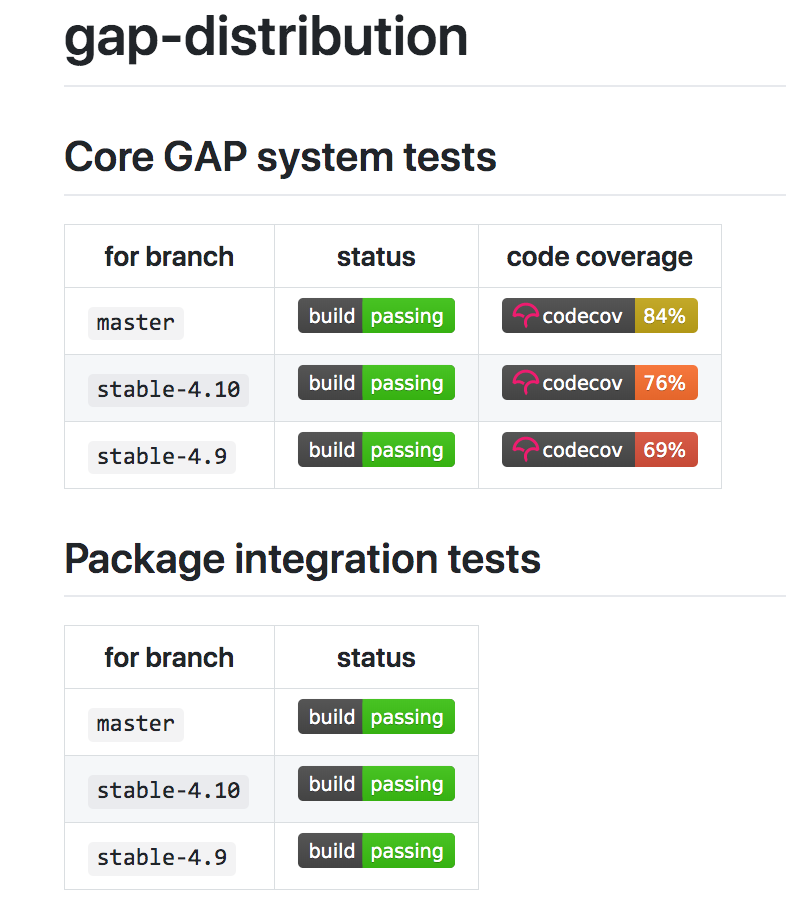
\includegraphics[width=5cm]{images/gap-core-tests}
    \caption{Dashboard with core GAP system and package integration tests}
    \label{fig:gap-core-tests}
\end{figure}

\subsection{Docker containers for testing, using and sharing GAP code}\label{docker}

We continued to maintain and expand the range of Docker containers,
initially reported in D3.1 and then in D3.8. Our main applications of
these containers are:
\begin{itemize}
\item speeding up regression tests by running container-based jobs on Travis CI;
\item sharing reproducible experiments in GAP Jupyter notebooks running on
  Binder (see Appendices~\ref{sec:repro-gap} and
  \ref{sec:libsemigroups-notebook});
\item as an alternative distributions,
  in particular this helps users who may not have administrator access
  to their systems, to access packages that they cannot run otherwise
  (e.g. due to missing dependencies or incompatibility with the operating system).
\end{itemize}

\begin{figure}[!ht]
    \centering
    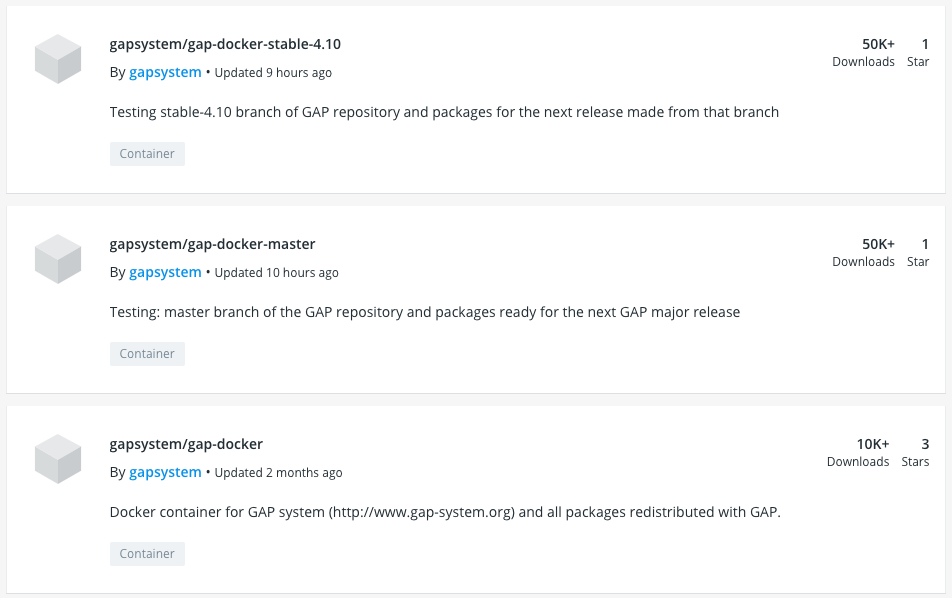
\includegraphics[width=12cm]{images/gap-docker}oif
    \caption{Selected \GAP Docker containers on Docker Hub}
    \label{fig:gap-docker}
\end{figure}

These containers are publicly available on Docker Hub (see Figure~\ref{fig:gap-docker}).
Containers with the development versions of \GAP and packages are updated daily, and have
the largest number of downloads since they are regularly used for testing. An example of
a test using such container could be found under ``Package integration tests'' on
Figure~\ref{fig:gap-core-tests}. Clicking on the ``status'' button leads to the overview displayed
in Figure~\ref{fig:gap-docker-master-testsuite}, from where one could inspect
test output for each of the configurations. 

\begin{figure}[!ht]
    \centering
    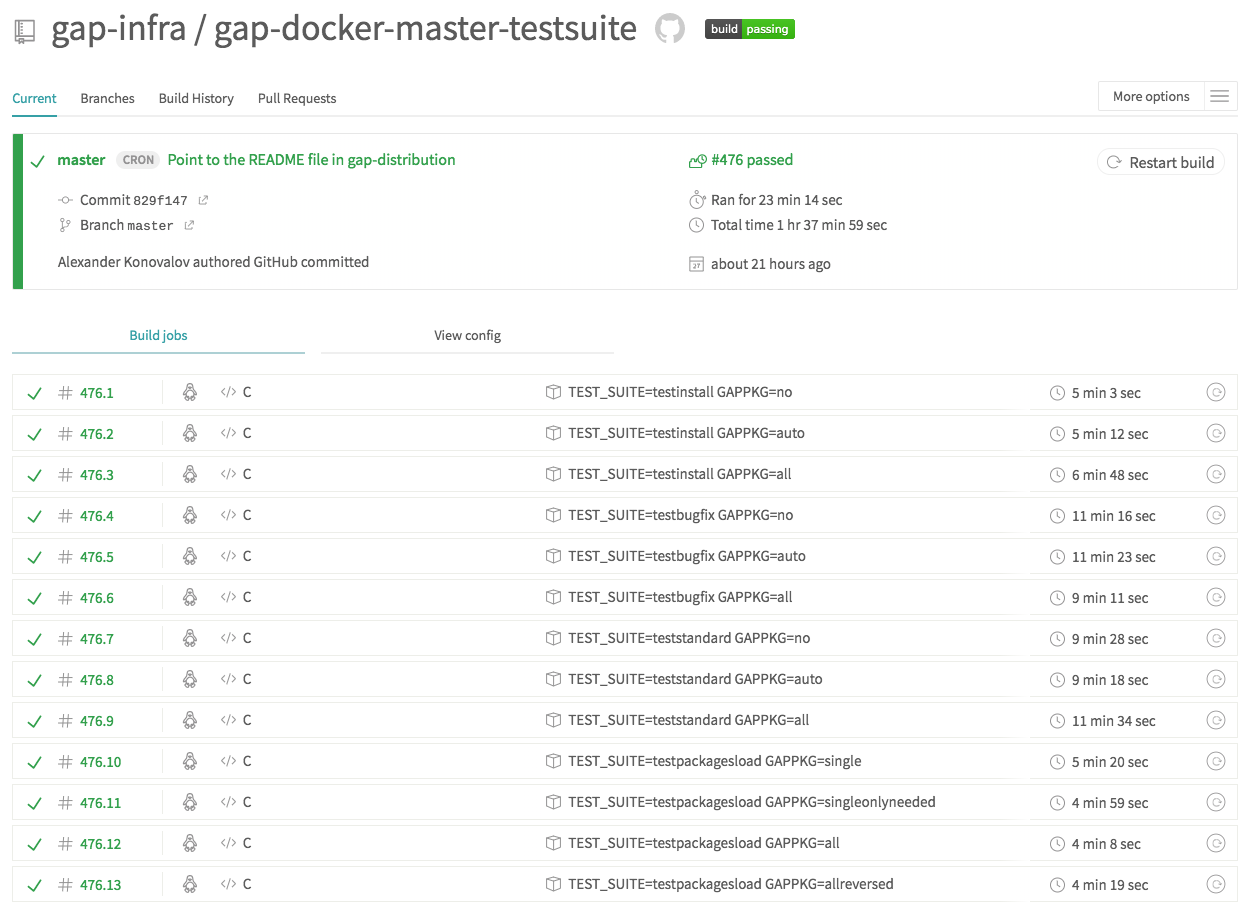
\includegraphics[width=\textwidth]{images/gap-docker-master-testsuite}
    \caption{GAP package integration tests on Travis CI}
    \label{fig:gap-docker-master-testsuite}
\end{figure}

%We made use of \href{https://travis-ci.org/}{Travis CI} and
%\href{https://www.appveyor.com/}{AppVeyor} which are 
%free (for open source projects) continuous integration platforms 
%that can be used to build and test software projects hosted at GitHub.
%\emph{Continuous Integration}, usually abbreviated as {\bf CI} is the process
%automated building and testing for every performed or suggested changes to 
%the source code repository. Using Travis and AppVeyor, one can test changes proposed
%in a pull request \emph{before} they are merged into the main repository.
%At the moment, we use Travis CI for tests on Linux and OS X, and 
%AppVeyor for tests on Windows.

%In addition to that, we started to use \href{https://codecov.io/}{Codecov}
%platform to collect \emph{code coverage} reports for GAP to ensure that our
%regression tests exercise GAP codebase at an acceptable level, and then
%the changes which are submitted via pull request are actually being tested
%by Travis CI. Making these results easily obtainable and publicly available
%had a great effect on the community. Adding new tests to improve code coverage
%is a useful task for new contributors to familiarize themselves with the
%project setup. Making coverage reports available for each pull requests
%facilitates checking code coverage during code review and
%encourages their authors to ensure that their contributions have a good
%quality and their suggested changes are actually being tested. 




%%A crucial role in these developments was played by the enhanced
%%profiling facilities discussed 
%%in Subsection~\ref{gap-4.8}. 
%%GAP~4.8 also introduced the {\tt TestDirectory} function to find
%%(recursively) all {\tt .tst} files from a given directory or a list of 
%%directories and run them using {\tt Test}. Having ability to test
%%changes more efficiently also allowed us to further improve all 
%%tools involved in testing, making their output more informative,
%%and allowing test integration into various automated workflows
%%by a better detection of the test outcomes. 
% the logic seems backwards here. Better test tools let us test better, not v.v.
% What I had in mind was that once we set up the system with the
% state of the testing framework as it was, we were able to "test the testing"
% itself, and improve it - for example, by adding progress indicators,
% report time spent on GC and memory used, etc.




\subsection{Continuous Testing of Package Cross Compatibility Ahead of
\GAP Releases}\label{pkg-update}
For packages redistributed with \GAP, our automatic package update system
checks regularly for new versions on the authors web pages, retrieves them, and then uses them in a
number of checks to ensure that new package releases are compatible with
each other and do not break the functionality of the core \GAP system. The
same process also helps us to check that changes in the core \GAP system
do not break the functionality of the packages redistributed with \GAP.
%% (provided those packages have standard tests that allow us to do that
%% automatically)
This system has dramatically simplified the process of making a \GAP
release or update, for which we need a mutually compatible set of
package versions, also compatible with the new core system. This used
to require extensive negotiation with package authors, and sometimes
took months, even though the number of packages was much smaller. Now
developers have continuous visibility of the functionality and
compatibility of released and upcoming versions of packages and of the
core system, and releases are much faster, delivering new features to
end users without compromising speed of delivery or robustness.

\subsection{Improvements to \GAP Package Tools}\label{sec:package-tools}

Sections \ref{sec:packages} and \ref{meataxe64} among others have shown
that developments important to our goal of a flexible, widely portable high performance
mathematical software system can increasingly occur in packages, as
well as in the core \GAP system. For that reason, as well as pursuit
of the broader goals of \ODK to support a user/developer community, we have attached
considerable priority to a supporting and promoting a healthy \GAP
package ecosystem. We have supported this through the developments
described in subsection~\ref{testing}, together with community
supporting activities described in D2.15, with
good effect. During the \ODK
project we have observed rapid growth of the number of \GAP packages
and of the number of active package
authors as well as steady improvements in the quality of package testing and more frequent
package updates. This has both been supported by, and encouraged, the
development of a wide range of tools to help package authors.

In this section introduce these tools and discuss the
impact which they had on the package ecosystem together with the increased
adoption of the open development model by package authors,

\subsubsection{ReleaseTools and GitHubPagesForGAP}
Our collaborator Max Horn (University of Siegen) developed
{\sf ReleaseTools}\footnote{\url{https://github.com/gap-system/ReleaseTools/}}
and {\sf GitHubPagesForGAP}\footnote{\url{https://github.com/gap-system/GitHubPagesForGAP/}}
which allow package
authors to fully automate the release procedure of a \GAP package hosted on GitHub
and the maintenance of a website for it hosted on GitHub pages,
reducing the time needed to publish it to a matter of minutes.

\subsubsection{The Example Package}
The \GAP package {\sf Example} by Werner Nickel, Greg Gamble and
Alexander Konovalov \cite{example}, which acts as a package template,
has been consistently maintained to track the development of
the packages infrastructure and serves to demonstrate a model use of modern
development tools.
%It switched to using {\tt TestDirectory} to demonstrate how to use 
%multiple test files in a GAP package, and migrated
%to GitHub, using {\sf ReleaseTools/GitHubPagesForGAP}
%for new releases. The guidance for package authors, formerly offered
%as an appendix to the {\sf Example} package manual, was moved to the GAP
%Reference manual in \GAP~4.9 release. Finally, the {\sf Example} package
%demonstrates how to set up Travis CI and CodeCov. Package authors
%may copy its configuration files and adapt them with minimal changes.

\subsubsection{PackageMaker}
To offer an alternative way to create a package,
Max Horn developed a GAP package called
{\sf PackageMaker}\footnote{\url{https://github.com/gap-system/PackageMaker}}
(not yet redistributed with \GAP),
which provides an interactive  ``package wizard''. This allows a
user to fill in the basic details 
of the intended package and then creates all of the files making up
the basic structure of the package. A particularly relevant
strength of this tool is that it hides the additional complexities of
packages which include C or C++ code, removing a barrier to faster implementation
of key kernels.

\subsubsection{AutoDoc}
\GAP packages are required to provide documentation.  The key central
format for \GAP documentation is XML-based, defined in the {\sf
  GAPDoc} package, and while convenient in many ways, can be rather
cumbersome and error prone to write by hand.
In 2012 Sebastian Gutsche 
and Max Horn (both now at the University of Siegen) developed the 
{\sf AutoDoc} package \cite{autodoc} which creates
documentation from simple structured comments in the source code,
similar to pydoc or javadoc.

By now, {\sf AutoDoc} has become very reliable and configurable, and
is in use by 89 GAP packages.
% for building some parts or their whole manuals.
% the number 89 was determined by 
%
% grep 'AutoDoc(' */makedoc.g | wc -l
%
% a note "parts or their whole manuals" is essential - 
% it is possible to build a GAPDoc manual using AutoDoc
% and automatically generate title page, updating the
% metadata from those in PackageInfo.g, avoiding the need
% to duplicate details in two places. The rest of the
% manuals for such packages may still remain in XML.

\subsubsection{Continuous Integration Support for Package Authors}
Using Docker containers described in Section~\ref{sec:gap-infra}
and shown on Figure~\ref{fig:gap-docker} enabled us to make the
results of regression tests for \GAP packages publicly
available via Travis CI. Using a prebuilt docker image 
greatly reduced the runtime of the test and allowed us to
have a separate test configuration for each package,
which is easily discover-able via the Travis CI interface.

Figure~\ref{fig:gap-docker-pkg-tests} shows a fragment of the dashboard
from \url{https://github.com/gap-system/gap-distribution} which 
indicates tests status. In this snapshot, it happens that a package
was depending on undefined behaviour of a \GAP library function, which
was changed, resulting in package tests failing. The prompt detection
of this interaction made it easy to diagnose and 
the author was immediately notified and reacted with a quick
fix. Previously this could have required many weeks of tedious
correspondence to resolve.


% \comment{this must be clear from picture}
%We separate passing and failing tests into different
%Travis jobs, and use that to monitor their status and check that
%changes in GAP do not break package tests. 

\begin{figure}[!ht]
    \centering
    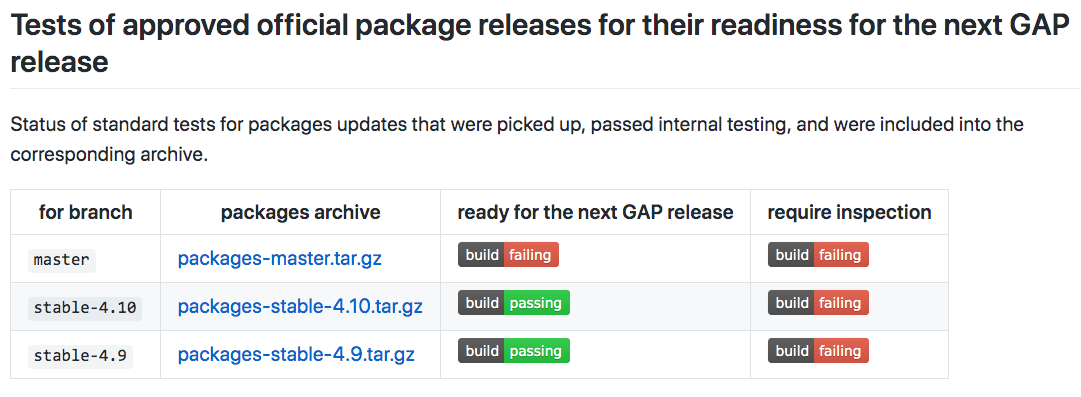
\includegraphics[width=\textwidth]{images/gap-docker-pkg-tests}
    \caption{Dashboard for Travis tests of \GAP packages (GitHub view)}
    \label{fig:gap-docker-pkg-tests}
\end{figure}


%% \comment{not sure if  Figure~\ref{fig:gap-infra-travis} adds anything new
%% - may be deleted?}
%% The setup for such tests is organized in the gap-infra GitHub organisation
%% (\url{https://github.com/gap-infra}. Figure~\ref{fig:gap-infra-travis} shows a 
%% screenshot of a dashboard which indicates tests status.
%% \comment{All these screenshots may be superfluous - I made them to show
%% what could be included, we can remove some or cut parts of them out later}

%% \begin{figure}[!ht]
%%     \centering
%%     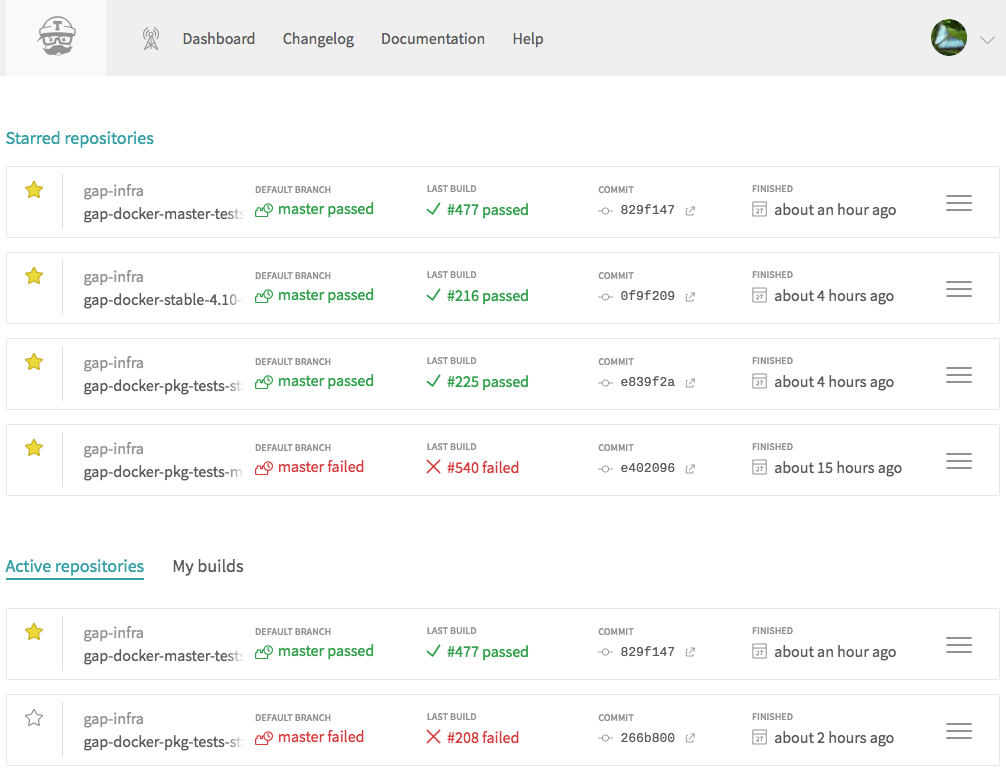
\includegraphics[width=\textwidth]{images/gap-infra-travis}
%%     \caption{Dashboard for Travis tests of \GAP packages (Travis CI view)}
%%     \label{fig:gap-infra-travis}
%% \end{figure}

% \comment{this may be too technical -- no I like it SL}
One of the extensions of the package testing framework, greatly 
facilitated by packages migrating to GitHub, was adding tests not
only for the latest official releases of GAP packages, but also
for their \emph{development} versions.
% https://travis-ci.org/gap-infra/gap-docker-pkg-tests-stable-4.10-devel
% https://travis-ci.org/gap-infra/gap-docker-pkg-tests-master-devel
In this case, the onus to check test outcomes is on package authors,
but they are able to quickly see how the changes that they have made to
a package but not released yet work in different settings (the
released and development versions of \GAP, with various different
combinations of other packages, for instance). Again this leads to
prompt diagnosis and easy fixing of problems, and improves the quality
of released packages.

%% Figure~\ref{fig:gap-packages-travis} shows a screenshot of a 
%% report on the activity in the gap-packages organization 
%% for the last month (for the current version of 
%% this report, check \url{https://travis-ci.org/gap-packages?tab=insights}).

%% \begin{figure}[!ht]
%%     \centering
%%     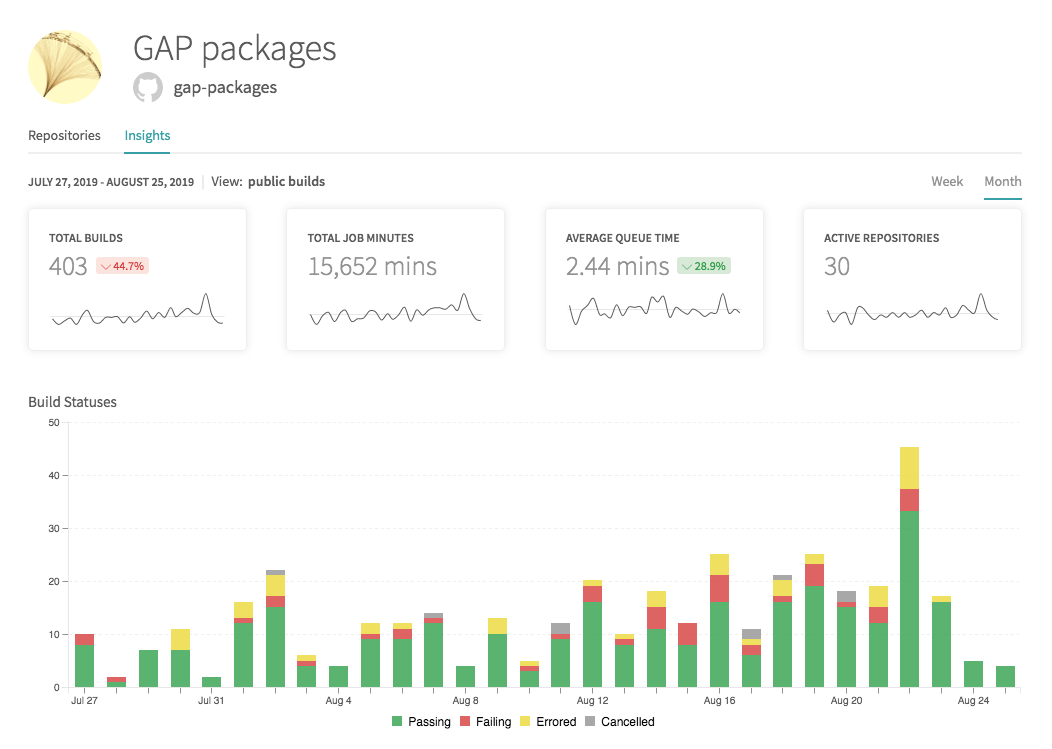
\includegraphics[width=\textwidth]{images/gap-packages-travis}
%%     \caption{Activity of Travis tests in gap-packages GitHub organization}
%%     \label{fig:gap-packages-travis}
%% \end{figure}

Finally, Figure~\ref{fig:gap-packages-codecov} show the code coverage
leaderboard. We aim at ensuring that code coverage for packages is 
not worse than for the core GAP system, but in fact many packages
put a lot of effort in ensuring that their coverage is close to 100\%. 

\begin{figure}[!ht]
    \centering
    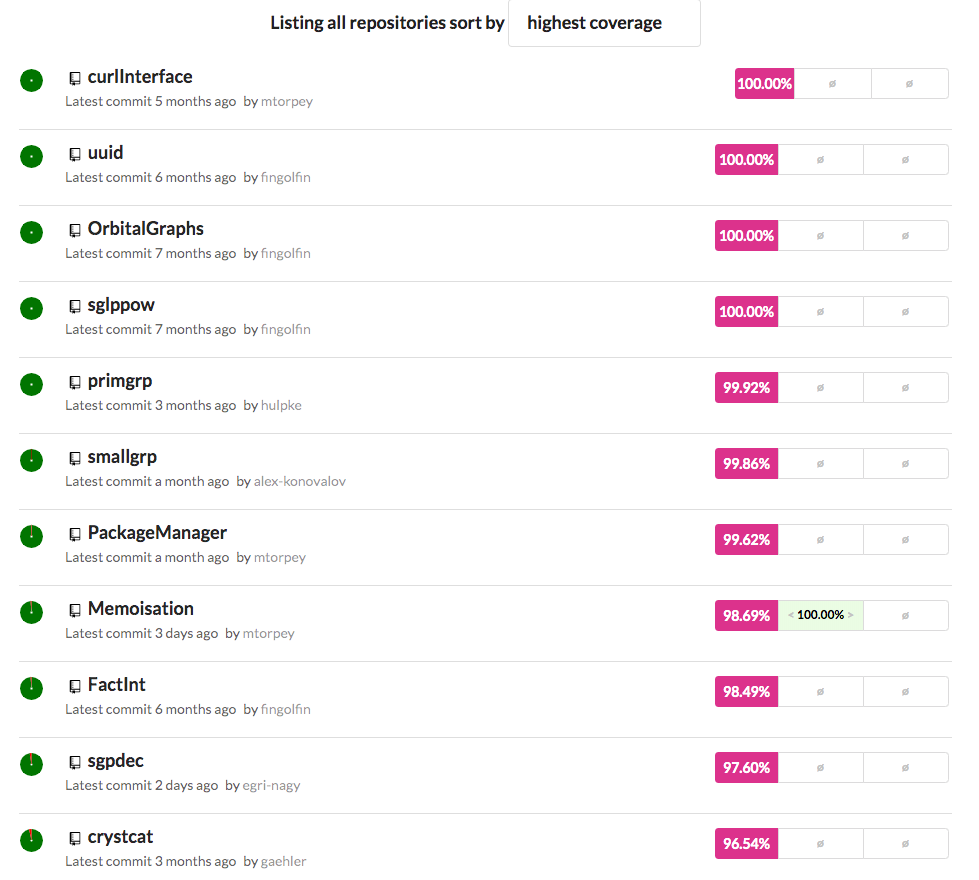
\includegraphics[width=\textwidth]{images/gap-packages-codecov}
    \caption{Codecov leaderboard for in gap-packages GitHub organization}
    \label{fig:gap-packages-codecov}
\end{figure}

\subsection{Open Development of \GAP Packages -- Measure of Uptake
  and Quality}\label{sec:uptake}

As we have explained above, we encourage and support package authors
to use open development models and tools similar to those used for
\GAP itself, since we believe that this is the best way to support the
development of a large portfolio of high quality compatible packages
which meet our users diverse computational requirements.

The openness of our preferred model also provides a number of tools
that we can use to measure our success, both in encouraging uptake and
in some aspects of the quality of the packages.

At the time of writing only 4 packages redistributed with GAP do not
have a public source code repository (to compare, in Month 38 there
were still 23 such packages). In some cases, this required significant
efforts on our part to establish contacts with authors who left
academia, gain their permission and agree a suitable license. We then
had to  populate a repository with a history based on archives of
past releases. In these cases (where we deem the package important
enough,  we formally ``adopt'' the package and declare it to be collectively maintained
by the GAP Group. This work helps ensure that the code will be
preserved in a usable state as \GAP and other tools evolve, something
that is
necessary to check and reproduce computational results. It also gives
visibility to the packages, sometimes attracting new contributors or
even maintainers. As
Figure~\ref{fig:gap-package-tests} shows, the number of individuals
involved in package development increased from 158 in Month 3 to 196
in Month 46.

Figure~\ref{fig:gap-package-releases} shows the number of \GAP packages
included in some \GAP release by year (of the release).
At the beginning of the project, GAP 4.7.9 published in November
2015 included 119 packages, 52\% of which had published a release in 2014--2015.
Now, GAP 4.10.2 includes 145 packages, 88\% of which have published a
release in 2018--2019. The ``long tail'' of packages that haven't been updated for
a long time is gradually reducing, a very encouraging sign of the
vigour of the community.
%(we take measures of not breaking
%existing functionality, but old packages are usually not picking up
%new improvements; and may prevent us from withdrawing obsolete
%functionality).

Larger proportion of recent releases means that 
packages are updated to make use of the recent \GAP developments,
and are responsive to reports about detected problems.
This is greatly facilitated by hosting packages on GitHub making it
easy and convenient for \GAP developers to offer support in the form
of code patches (``pull requests'' in git terminology) or even by
actually publishing releases for them.
%who prefer to overlook mathematical functionality and general development of the
%package but do not want to dive into technicalities of release wrapping.

\begin{figure}[!ht]
    \centering
    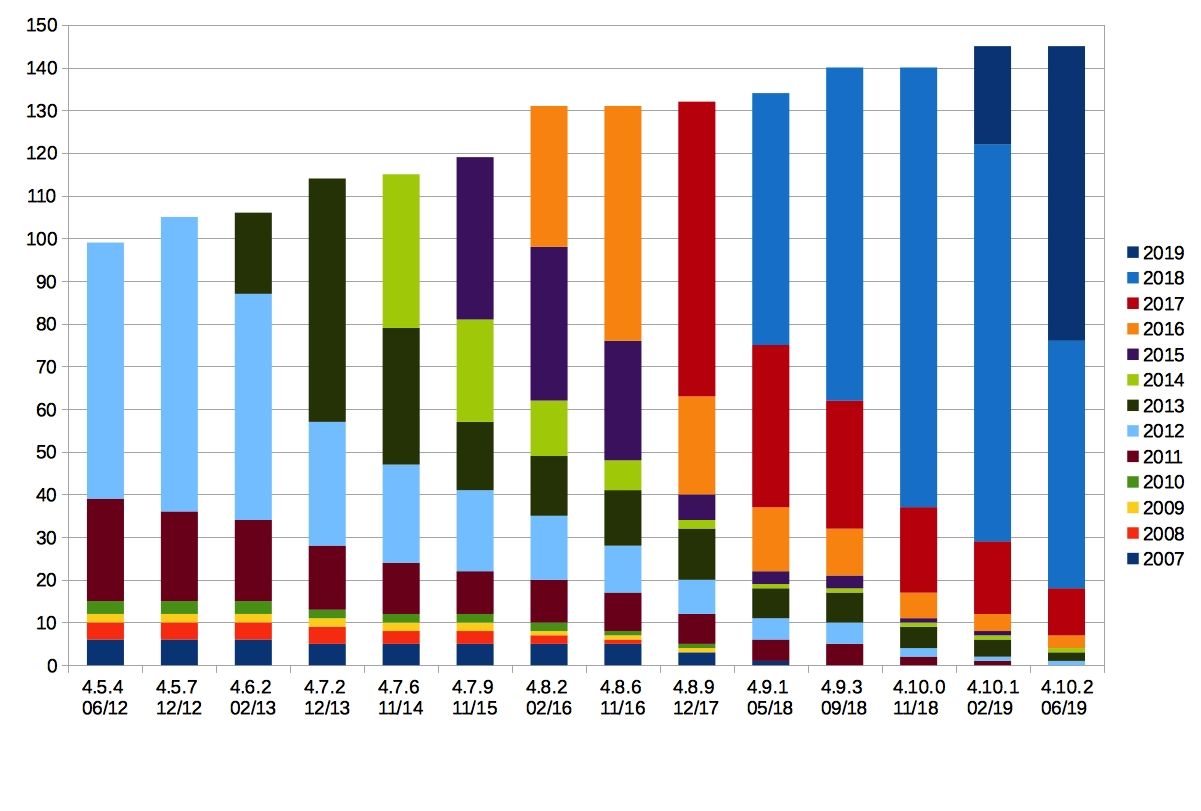
\includegraphics[width=\textwidth]{images/gap-package-releases}
    \caption{Number of \GAP packages and their release year}
    \label{fig:gap-package-releases}
\end{figure}


Over the same period, package releases not only became more frequent,
but their quality also 
improved. In November 2015, 52\% of packages did not provide a standard 
test suite at all, whereas now 78\% of packages have one.
% https://github.com/gap-packages/gap-packages.github.io/issues/9
It is then easy for their authors to  regularly test them 
with published GAP releases and with the development version.
Some have their own continuous integration systems
(e.g. the \href{https://homalg-project.github.io/}{\sf homalg} project,
which uses \href{https://circleci.com/}{CircleCI}).
At the moment of writing, in the stable-4.10 branch,
standard tests pass for 102 packages
% https://travis-ci.org/gap-infra/gap-docker-pkg-tests-stable-4.10
and fail for 12.
% https://travis-ci.org/gap-infra/gap-docker-pkg-tests-stable-4.10-staging 
These failures are probably not serious bugs but variations in output
format, or an incompatibility with some other package
that is not loaded by default).

\begin{figure}[!ht]
    \centering
    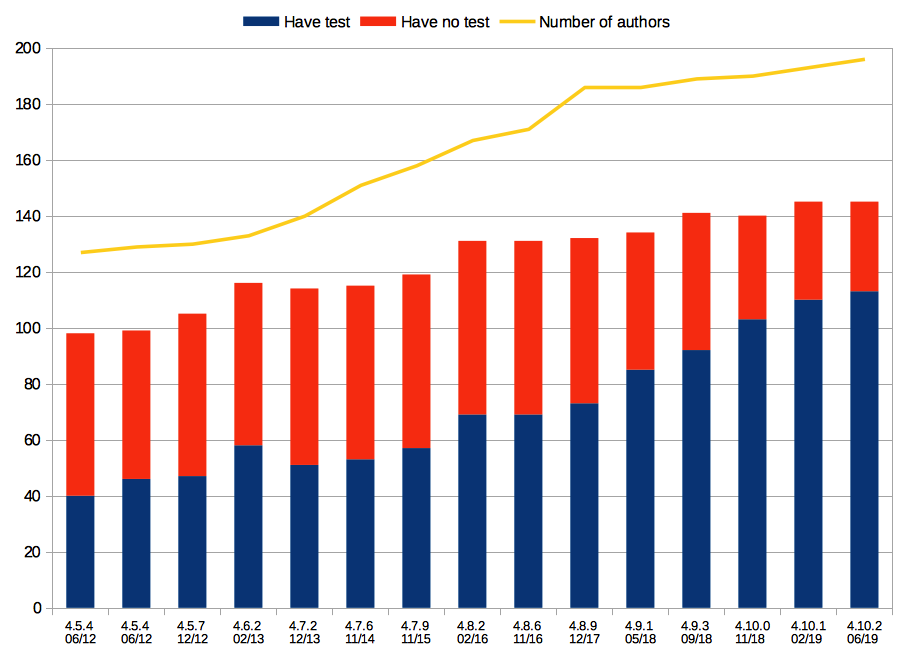
\includegraphics[width=\textwidth]{images/gap-package-tests}
    \caption{Number of \GAP packages, their authors, and packages with tests.}
    \label{fig:gap-package-tests}
\end{figure}

% grep github currentPackageInfoURLList | wc -l
Another illustrative statistics is the number of \GAP packages
whose websites hosted on GitHub pages (some of them use
their own setup, different from {\sf GitHubPagesForGAP}. This is not a
specific suggestion or requirement, but it indicates engagement with
open development  methods, and makes it easy to keep the website up to date.
The following table gives this number for August of each respective year:

\begin{center}
\begin{tabular}{| c | c | c | c | c | c |} 
\hline
Year & 2015 & 2016 & 2017 & 2018 & 2019 \\
\hline
Number of packages & 14 & 45 & 61 & 92 & 124 \\
\hline
\end{tabular}
\end{center}

\subsection{The \GAP package manager}\label{pkg-manager}

\subsubsection{Background}

For many years, the installation of packages in \GAP has been an
entirely manual process.  If a user requires a package that is not
currently installed on their system, they are required to visit the
\GAP website, or the website of the required package, download an
archive or repository and extract it into their package directory.  In
many cases, they must also compile C code or external programs
within the package before use, in a process that is not consistent
between packages.  Worst of all, any packages on which their chosen
package depends must also be installed individually, including all
these steps for each one.

This awkward installation procedure is mitigated by the inclusion of a
large number of packages with the main release archive, which solution
masks the problem for the majority of users, who do not require any
more specialized packages.  However, it also results in a 1.6 GB
standard installation, of which the packages make up 1.4 GB, and while
the files are installed, C code often does not get compiled. While
some packages are used by almost every \GAP user because they enhance
the performance of core \GAP features, only a subset of the others
will be needed by any specific end user. This need may be explicit (when
they load a package relevant to their research interests) or implicit
(to satisfy package dependencies). It would be desirable to avoid all
users having copies of all packages by default.

Additional problems can arise when the \GAP installation is controlled
by central administration and a user needs an extra package installed or a
package compiled, or when a user wishes to update to a new package
version ahead of it being included in a new \GAP distribution.


In the light of these issues, the possibility of a more sophisticated
package management system for \GAP has been discussed for some time,
and was realized with the creation of {\sf PackageManager}
\cite{PackageManager} in Month 37, by Michael Torpey.  Development
started after a discussion at \GAP Days Fall 2018
(\url{https://www.gapdays.de/gapdays2018-fall/}) and an initial
release was made before the end of that meeting.  New features have
been added in various further releases across the past year.

\subsubsection{Design}

{\sf PackageManager} is a \GAP package itself, and is utilized in the
standard way, by loading it into a \GAP session and executing \GAP
functions. This approach to package management was chosen over an external
manager since it allows users to install and remove packages without ever
leaving the \GAP prompt, while making no, or minimal assumptions about
the underlying system setup. This gives
users a comfortable and familiar environment. In most cases, packages can be installed
and loaded without restarting the session, as shown in Figure \ref{fig:pkgman-sample-b}.
This means that users' workflow is interrupted as little as possible, and they do
not need to save and reload their work.

\begin{figure}[!ht]
  \begin{mdframed}
    \centering
    {\tiny
\begin{verbatim}
gap> InstallPackage("digraphs");
#I  Getting PackageInfo URLs...
#I  Retrieving PackageInfo.g from https://gap-packages.github.io/Digraphs/PackageInfo.g ...
#I  Downloading archive from URL https://github.com/gap-packages/Digraphs/releases/download\
/v0.15.4/digraphs-0.15.4.tar.gz ...
#I  Saved archive to /tmp/tmcLM2FI/digraphs-0.15.4.tar.gz
#I  Extracting to /home/user/.gap/pkg/digraphs-0.15.4 ...
#I  Checking dependencies for Digraphs...
#I    io >=4.5.1: true
#I    orb >=4.8.2: true
#I  Running compilation script on /home/user/.gap/pkg/digraphs-0.15.4 ...
true
gap> LoadPackage("digraphs", false);
true
\end{verbatim}
    }
    \end{mdframed}
    \caption{Installing a package using {\sf PackageManager}.}
    \label{fig:pkgman-sample-b}
\end{figure}

The most important function provided by {\sf PackageManager} is
\texttt{InstallPackage}, which can take as argument the URL of an archive, repository, or package info file, or simply the
name of a package.  In the case of a URL, the appropriate file is retrieved
using an internet connection, and used to install the package; if a package name
is given, it is looked up in a pre-defined list of package URLs and installed
from there.  In most cases, the latest released version of a package is
installed, but a user can specify an older version by giving an explicit archive
URL, or a development version by specifying a branch in a
version control repository.
Also provided are \texttt{RemovePackage} and \texttt{UpdatePackage}, which
remove a package or update a package to the latest version, given the package's
name.

The ability to install a package given only its name is useful, but requires
some important design decisions: how do we decide which packages to support, and
which versions do we install by default?  One option would be to have a
centralized repository (as is common for the {\sf APT} package manager) which
contains a carefully checked set of package versions that are known to work with
the installed version of \GAP and with each other; this has the advantage of
stability and control, but may make it harder to get the latest software
versions.  The other option is to store links to appropriate locations on the
package websites, allowing the most recently released version to be installed
without explicit approval from the \GAP authors; this approach is closer to the
more liberal {\sf pip} package manager for the Python language.
In the end, the latter approach was taken for the following reasons:
\begin{itemize}
\item approved package versions for a given release are likely to be included
  with the \GAP installation anyway, and it is unlikely that users would need
  to reinstall these;
\item the latter approach requires no additional infrastructure, since a
  list of URLs for package info files is already maintained for testing purposes;
\item this approach encourages active use, and therefore testing, of recent releases.
\end{itemize}
This decentralized approach has therefore been adopted for the moment, though
future development could move easily towards a different approach.

\subsubsection{Features}

Over the course of {\sf PackageManager}'s development, it has accumulated
various features that automate as much of the installation process as possible.
During installation, the following operations are carried out automatically:
\begin{itemize}
\item any kernel module is configured and compiled, if present;
\item package documentation is built from source if necessary;
\item external software prerequisites are installed using a package-specific
  shell script, if one is present;
\item all missing package dependencies are installed, or recompiled if broken;
\item basic checks are performed to verify that installation was successful.
\end{itemize}

The new packages are installed in a user-specific directory separate
from the \GAP installation, so that multiple users on a shared system
can have distinct package configurations. The packages will also
remain present if the main \GAP installation is moved or replaced.

This has resulted in a reasonably smooth installation process, with very little
friction encountered by a user who tries to get a new package working.
The package manager is
now a deposited package in \GAP, and is therefore distributed in the main
archive with each release.


\subsubsection{Best practice}

{\sf PackageManager} was written using modern open-source software technologies
and practices.  In the report on OpenDreamKit D1.5, in Section 4.3.2, there are
two checklists for best practices: one for software engineering, and one for
dissemination.  The package fulfills all the requirements in both lists, as summarized in
Tables \ref{tab:pkgman-se-check} and \ref{tab:pkgman-diss-check}.

\begin{table}[ht]
  \renewcommand{\arraystretch}{1.2}
  \begin{tabular}{|p{5.1cm}|c|p{9.5cm}|}\hline
    Version control & \checkmark & Git \\ \hline
    Tests & \checkmark & \multirow{2}{*}{\GAP test suite with 99\% code coverage} \\ \cline{1-2}
    Automated tests & \checkmark & \\ \hline
    Continuous integration & \checkmark & Travis runs test suite for every commit \\ \hline
    Automatic building of releases & \checkmark & {\sf ReleaseTools} (see above) \\ \hline
  \end{tabular}
  \vspace{0pt}
  \caption{Software engineering good practice checklist for {\sf PackageManager}}
  \label{tab:pkgman-se-check}
\end{table}

\begin{table}[ht]
  \renewcommand{\arraystretch}{1.2}
  \begin{tabular}{|p{5.1cm}|c|p{9.5cm}|}\hline
    Host code publicly & \checkmark & \url{https://github.com/gap-packages/PackageManager} \\ \hline
    Reference Manual (APIs) & \checkmark & GAPDoc/Autodoc, and hosted on package website \\ \hline
    Tutorial (for beginning users) & \checkmark & \multirow{2}{9.5cm}{Quick examples in readme and manual, before more detailed documentation} \\ \cline{1-2}
    Examples & \checkmark & \\ \hline
    Live interactive online demos & \checkmark & Binder link included in readme \\ \hline
    Support mechanisms & \checkmark & Github issues \\ \hline
    How to cite the output? & \checkmark & Explained on readme and website \\ \hline
    Installation mechanism & \checkmark & Distributed with \GAP, and can update itself \\ \hline
    High level description accessible to non-experts & \checkmark & In readme, and chapter 1 of manual \\ \hline
    URLs/Blog/etc to and from OpenDreamKit project & \checkmark & OpenDreamKit link and logo in readme \\ \hline
    Grant acknowledgments & \checkmark & Acknowledged in readme \\ \hline
    Open Source license & \checkmark & GPL v2 or later \\ \hline
    Workshop & \checkmark & \multirow{2}{9.6cm}{Demos in \textit{CIRCA Seminar} (USTAN, Month 43) and \textit{Workshop on Mathematical Data} (Cernay, Month 48)} \\ \cline{1-2}
    Engaging users & \checkmark & \\ \hline
  \end{tabular}
  \vspace{0pt}
  \caption{Dissemination good practice checklist for {\sf PackageManager}}
  \label{tab:pkgman-diss-check}
\end{table}

\subsubsection{Other uses}

Aside from making the on-demand installation of individual packages easier, {\sf
  PackageManager} has implications for the future of how \GAP is distributed.
There are no current plans to stop distributing
deposited packages with the \GAP archive by default, but the
possibility of distribute a much smaller archive, containing only a few
fundamental packages and {\sf
  PackageManager} itself and then installing others as needed is now
opened up.  Furthermore, the package manager
can be used by other systems that interact with \GAP to manage
their \GAP installations more easily.  The \cocalc system now contains {\sf PackageManager}
as part of its \GAP 4.10.2 installation, enabling each user to install any
packages they need without \cocalc operators being forced to manage these
installations separately.  This is an example of positive two-way interaction
with \cocalc, and sets as a good precedent for interaction with other
systems.


